\section{Evaluation Protocol}

\paragraph{Visit chains and geometry.}
The real room contains visits A, B, and C; the simulated apartment and Flat contain visits A and B.
Each method continues through the chain using its own map updates. Panoptic Multi-TSDFs loads the preceding
visit's map through its native interface. Geometry is evaluated at the end of each visit, before global
refinement of Gaussian maps. The real-room reference is a reconstructed surface at 1\,cm resolution,
restricted to the room. The synthetic reference consists of ground-truth surfaces observed up to the evaluation
time. Thus the reference includes previously observed regions that the current visit does not see.
\Cref{tab:supp_geometry} reports every visit; \cref{tab:supp_restart} additionally compares native maps rebuilt
from scratch with our continuously updated maps.

% Generated from experiments_rewrite_20261101/results.json
\begin{table*}[t]
\centering
\fontsize{9}{10.3}\selectfont
\setlength{\tabcolsep}{5pt}
\renewcommand{\arraystretch}{1.08}
\begin{tabular}{@{}l*{8}{r}@{}}
\toprule
& \multicolumn{3}{c}{Real} & \multicolumn{2}{c}{Synthetic} & \multicolumn{2}{c}{Flat} & 3RScan \\
\cmidrule(lr){2-4}\cmidrule(lr){5-6}\cmidrule(lr){7-8}
Method & A & B & C & A & B & A & B & Mean \\ \midrule
Khronos & 90.8 & 88.9 & 87.7 & 93.6 & 93.1 & 86.0 & 86.9 & 88.8 \\
Panoptic & 82.6 & 86.2 & 87.3 & 90.3 & 90.5 & 85.1 & 89.4 & 81.0 \\
Ours (TSDF) & 94.6 & 96.2 & 96.1 & 99.2 & 99.2 & 86.5 & 90.1 & 91.8 \\
\midrule
GaME & 91.9 & 88.6 & 90.1 & 94.3 & 91.2 & 86.6 & 87.4 & 87.0 \\
Ours (3DGS) & 93.5 & 93.1 & 95.0 & 97.7 & 96.6 & 86.3 & 89.8 & 89.7 \\
\midrule
wavemap & 87.2 & 81.2 & 84.5 & 92.2 & 93.2 & 79.5 & 80.2 & 75.6 \\
Ours (Occ.) & 87.9 & 89.1 & 91.0 & 92.4 & 94.2 & 79.5 & 82.4 & 79.4 \\
\bottomrule
\end{tabular}
\caption{\textbf{Geometry at every visit.} F1 at 5\,cm (\%, $\uparrow$); 3RScan uses the room-wise averaging described in the text.}
\label{tab:supp_geometry}
\end{table*}

% Generated from experiments_rewrite_20261101/results.json
\begin{table*}[t]
\centering
\fontsize{9}{10.3}\selectfont
\setlength{\tabcolsep}{5pt}
\renewcommand{\arraystretch}{1.08}
\begin{tabular}{@{}lll*{6}{r}@{}}
\toprule
& & & \multicolumn{3}{c}{Native restart} & \multicolumn{3}{c}{Ours, continued} \\ \cmidrule(lr){4-6}\cmidrule(lr){7-9}
Dataset & Map & Visit & P & R & F1 & P & R & F1 \\ \midrule
Real & TSDF & A & 85.62 & 96.87 & 90.90 & 93.22 & 95.94 & 94.56 \\
 & TSDF & B & 93.71 & 98.28 & 95.94 & 94.93 & 97.47 & 96.18 \\
 & TSDF & C & 91.33 & 98.62 & 94.83 & 93.62 & 98.81 & 96.14 \\
 & 3DGS & A & 95.53 & 91.00 & 93.21 & 95.98 & 91.19 & 93.52 \\
 & 3DGS & B & 95.86 & 91.47 & 93.62 & 92.15 & 94.00 & 93.07 \\
 & 3DGS & C & 97.00 & 93.72 & 95.33 & 95.36 & 94.68 & 95.01 \\
 & Occupancy & A & 81.69 & 93.43 & 87.17 & 81.72 & 95.02 & 87.87 \\
 & Occupancy & B & 86.79 & 90.84 & 88.77 & 85.44 & 93.10 & 89.11 \\
 & Occupancy & C & 82.41 & 96.66 & 88.97 & 84.72 & 98.36 & 91.03 \\
\midrule
Synthetic & TSDF & A & 98.38 & 89.33 & 93.64 & 99.74 & 98.63 & 99.18 \\
 & TSDF & B & 98.10 & 77.57 & 86.63 & 99.80 & 98.66 & 99.23 \\
 & 3DGS & A & 94.02 & 95.85 & 94.92 & 97.01 & 98.49 & 97.74 \\
 & 3DGS & B & 93.30 & 78.72 & 85.39 & 97.15 & 95.99 & 96.57 \\
 & Occupancy & A & 93.00 & 91.48 & 92.24 & 93.13 & 91.68 & 92.40 \\
 & Occupancy & B & 96.49 & 76.50 & 85.34 & 94.90 & 93.58 & 94.23 \\
\bottomrule
\end{tabular}
\caption{\textbf{Restart versus continued mapping.} Precision, recall, and F1 at 5\,cm (\%). Native restart maps and our continued maps use the same visit-specific reference.}
\label{tab:supp_restart}
\end{table*}


\paragraph{Objects and changes.}
Object matching uses a 0.5\,m distance threshold throughout. Scores at successive snapshots are weighted by the
duration for which each snapshot is current. For 3RScan, scores are first averaged over visits within a room
and then over eight rooms. Change F1 pools true positives, false positives, and false negatives across the
complete chain; 3RScan contains 77 pooled reference events. These include appearances and disappearances
within visits and between visits.
The state-based 3RScan evaluator considers a reference state represented when at least half its points lie
within 10\,cm of a single mapped object surface. An earlier state that is no longer represented supplies
disappearance evidence; a new represented state supplies appearance evidence. A persistent reference object
reported as disappeared is a false positive.

\paragraph{Map exports.}
Evaluation reads each method's own decisions and map contents. Panoptic snapshots are recorded every 2\,s of
dataset time. Its New, Matched, and Persistent submaps are present; Absent submaps supply disappearance
decisions, while Unobserved submaps do not. Object geometry remains available to the evaluator for matching.
Gaussian and occupancy exports form object components using 26-connectivity on a 10\,cm grid within each
identity, accepting components of volume 0.005--10\,m$^3$, following the Khronos object construction settings.
The same export rule is used for a representation's native and proposed updates. State records in the chained
exports declare appearances; the exporter does not infer movement by counting closed states.

\paragraph{Inputs and native baselines.}
Khronos receives annotated instances on the real room, synthetic apartment, 3RScan, and TESSE; its Flat run
uses semantic input. Real-room and 3RScan instance tracking uses the supplied identities, while synthetic and
TESSE tracking uses mask overlap. Panoptic uses its dataset configurations: 5\,cm object resolution and
10\,cm background resolution for the synthetic apartment, and 5\,cm resolution on the real room and 3RScan.
GaME and wavemap continue with their native updates for the baseline rows. The GaME 3RScan run uses its
dataset-adapted implementation. On real RGB-D, invalid depths are excluded from geometry supervision and
allocation; the synthetic GaME adapter corrects relative-pose keyframe selection and guards sampling termination.
Flat uses the original GaME configuration.
For 3RScan, evaluation images are 480$\times$270 for both Gaussian methods. In three rooms, Gaussian mapping
uses 240$\times$135 inputs to fit memory; evaluation remains at 480$\times$270.

\paragraph{Rendering.}
Following GaME~\cite{yugay2026game}, every tenth frame of the final visit is held out, except the first frame.
PSNR, MS-SSIM, LPIPS with the AlexNet backbone, and measured-depth L1 are averaged over held-out frames.
The 3RScan result is the mean over the final visit of each of eight rooms. Gaussian geometry uses the
pre-refinement map; the rendering table uses the map after global refinement. The main benchmark and the
controlled Flat ablations retain their respective full-run results.

\paragraph{Integration settings.}
The common surface test uses a 5\,cm tolerance, a $60^\circ$ incidence limit~\cite{nguyen2012kinect}, and threshold $\ln 99$.
Each depth image requires at least $\min(30,\nu_{\mathrm{rel}})$ judged samples. The successor displacement
threshold is 10\,cm. Our TSDF uses 5\,cm voxels and a 10\,cm truncation band, Gaussian surface tests use a
5\,cm tolerance floor, and occupancy uses 5\,cm cells. These settings are shared across the reported datasets.

\section{Single-Run Spatio-Temporal Evaluation}

% Generated from experiments_rewrite_20261101/results.json
\begin{table*}[t]
\centering
\fontsize{9}{10.3}\selectfont
\setlength{\tabcolsep}{2.3pt}
\renewcommand{\arraystretch}{1.08}
\begin{tabular}{@{}ll*{13}{r}@{}}
\toprule
& & \multicolumn{3}{c}{Background} & \multicolumn{3}{c}{Static objects} & \multicolumn{3}{c}{Dynamic objects} & \multicolumn{3}{c}{Changes} & Geometry \\
\cmidrule(lr){3-5}\cmidrule(lr){6-8}\cmidrule(lr){9-11}\cmidrule(lr){12-14}
Scene & Method & P & R & F1 & P & R & F1 & P & R & F1 & P & R & F1 & F1 \\ \midrule
Office & Khronos & 93.8 & 66.0 & 74.6 & 99.3 & 57.0 & 69.0 & 97.3 & 75.5 & 84.8 & 9.2 & 49.3 & 43.6 & 92.8 \\
 & Ours & 95.3 & 67.5 & 76.1 & 99.1 & 57.4 & 69.5 & 100.0 & 97.5 & 98.7 & 94.4 & 50.4 & 79.0 & 94.2 \\
\midrule
Apartment & Khronos & 91.9 & 69.0 & 78.0 & 96.7 & 38.8 & 55.9 & 95.7 & 76.2 & 85.3 & 16.3 & 56.8 & 36.9 & 86.1 \\
 & Ours & 96.5 & 69.3 & 79.9 & 96.7 & 46.7 & 63.3 & 94.9 & 94.0 & 95.1 & 93.3 & 59.2 & 92.7 & 88.1 \\
\bottomrule
\end{tabular}
\caption{\textbf{Full TESSE evaluation.} Precision, recall, and F1 are official query-aggregated percentages. Final geometry uses F1 at 5\,cm.}
\label{tab:supp_tesse}
\end{table*}

% Generated from experiments_rewrite_20261101/results.json
\begin{table*}[t]
\centering
\fontsize{9}{10.3}\selectfont
\setlength{\tabcolsep}{2.3pt}
\renewcommand{\arraystretch}{1.08}
\begin{tabular}{@{}ll*{13}{r}@{}}
\toprule
& & \multicolumn{3}{c}{Background} & \multicolumn{3}{c}{Static objects} & \multicolumn{3}{c}{Dynamic objects} & \multicolumn{3}{c}{Changes} & Geometry \\
\cmidrule(lr){3-5}\cmidrule(lr){6-8}\cmidrule(lr){9-11}\cmidrule(lr){12-14}
Scene & Method & P & R & F1 & P & R & F1 & P & R & F1 & P & R & F1 & F1 \\ \midrule
Real A & Khronos & 88.7 & 76.2 & 80.6 & 99.0 & 90.6 & 94.3 & 0.0 & 0.0 & -- & 6.9 & 98.8 & 54.2 & 90.9 \\
 & Ours & 97.2 & 76.9 & 84.6 & 97.9 & 95.0 & 96.4 & 92.6 & 98.3 & 96.0 & 36.6 & 100.0 & 97.0 & 94.5 \\
\midrule
Real B & Khronos & 93.2 & 82.6 & 86.6 & 95.0 & 90.2 & 92.4 & 96.5 & 14.9 & 28.2 & 6.7 & 15.5 & 42.0 & 95.9 \\
 & Ours & 95.9 & 82.5 & 87.7 & 98.0 & 94.0 & 95.9 & 76.0 & 98.2 & 88.4 & 26.9 & 75.1 & 66.7 & 97.4 \\
\midrule
Real C & Khronos & 92.6 & 83.0 & 86.7 & 85.0 & 84.2 & 84.1 & 16.8 & 0.9 & 3.3 & 29.2 & 25.3 & 46.0 & 94.8 \\
 & Ours & 96.4 & 83.8 & 88.9 & 94.0 & 92.9 & 93.3 & 90.5 & 80.6 & 97.0 & 88.3 & 69.1 & 85.7 & 97.0 \\
\midrule
Synthetic A & Khronos & 95.3 & 64.8 & 77.0 & 63.9 & 78.2 & 69.5 & 1.7 & 0.4 & 0.9 & 31.0 & 85.9 & 63.5 & 93.6 \\
 & Ours & 98.1 & 87.3 & 92.1 & 72.5 & 82.8 & 77.0 & 100.0 & 43.7 & 73.6 & 52.9 & 45.9 & 71.3 & 99.2 \\
\midrule
Synthetic B & Khronos & 96.4 & 47.9 & 63.8 & 63.4 & 77.8 & 68.5 & 73.5 & 17.4 & 27.4 & 23.9 & 45.1 & 43.7 & 86.6 \\
 & Ours & 98.5 & 64.1 & 77.1 & 74.0 & 84.7 & 77.9 & 99.9 & 57.5 & 73.9 & 75.7 & 32.4 & 59.2 & 89.9 \\
\bottomrule
\end{tabular}
\caption{\textbf{Independent single-visit runs.} Precision, recall, and F1 are official query-aggregated percentages. Final geometry uses F1 at 5\,cm.}
\label{tab:supp_single}
\end{table*}


\paragraph{TESSE.}
We use the office and apartment sequences released with Khronos~\cite{schmid2024khronos}. Both methods use
5\,cm voxels. The official evaluator queries each saved map at preceding scene times and aggregates background,
static-object, dynamic-object, and change scores. \Cref{tab:supp_tesse} reports its precision, recall, and F1
outputs separately. We use a 5\,cm background matching tolerance; the original Khronos paper reports a
20\,cm tolerance. Our background export includes current and historical object geometry, matching the geometry
included in the Khronos background mesh. Final-map geometry is reported separately from the 4D aggregate.

\paragraph{Independent visits.}
\Cref{tab:supp_single} evaluates each real and synthetic visit from an empty map. The reference state sequence
is restricted to that visit: objects present at its start are initially present, and changes between visits are
excluded from its event set. Dynamic references are people in the real sequences and objects moved in front
of the camera in the synthetic sequences. Background, static objects, dynamics, and changes use the same
official query aggregation as TESSE. The final geometry column compares the last map with that visit's surface
reference and therefore differs from the historical background score.

\section{Complete Ablations}

% Generated from experiments_rewrite_20261101/results.json
\begin{table*}[t]
\centering
\fontsize{9}{10.3}\selectfont
\setlength{\tabcolsep}{2.7pt}
\renewcommand{\arraystretch}{1.08}
\begin{tabular}{@{}l*{9}{r}@{}}
\toprule
& \multicolumn{3}{c}{F1 ($\%$)} & \multicolumn{2}{c}{PSNR (dB)} & & & & Region \\
Variant & Geom. & Obj. & Chg. & Pre & Post & MS-S & LPIPS & L1 & PSNR \\ \midrule
\multicolumn{10}{@{}l}{\textit{Block a}} \\
\rowcolor{oursbg!45}
Full (a) & 90.00 & 66.77 & 83.33 & 23.78 & 27.63 & 0.947 & 0.117 & 0.48 & -- \\
w/o change decisions & 84.42 & 66.73 & 68.75 & 21.91 & 23.79 & 0.912 & 0.156 & 3.31 & -- \\
Object scope, no handover & 84.36 & 66.80 & 68.75 & 21.92 & 23.68 & 0.910 & 0.158 & 3.32 & -- \\
Object scope & 89.70 & 66.91 & 83.33 & 23.85 & 27.46 & 0.947 & 0.117 & 0.53 & -- \\
Local-surface scope & 89.60 & 66.56 & 80.00 & 23.92 & 27.88 & 0.950 & 0.114 & 0.48 & -- \\
w/o handover & 89.74 & 66.61 & 80.00 & 23.93 & 27.73 & 0.950 & 0.113 & 0.48 & -- \\
\midrule
\multicolumn{10}{@{}l}{\textit{Block b}} \\
\rowcolor{oursbg!45}
Full (b) & 89.81 & 66.46 & 83.33 & 23.95 & 27.77 & 0.950 & 0.115 & 0.45 & 28.13 \\
Unrestricted old frames & 86.19 & 66.67 & 83.33 & 21.50 & 22.69 & 0.891 & 0.174 & 3.66 & 17.45 \\
Unrestricted during refinement & 89.81 & 66.46 & 83.33 & 23.95 & 22.78 & 0.893 & 0.172 & 3.45 & 17.74 \\
Discard conflicting frames & 89.95 & 66.89 & 83.33 & 23.83 & 27.78 & 0.949 & 0.118 & 0.47 & 28.05 \\
Current-time map selection & 90.17 & 66.97 & 83.33 & 23.91 & 27.83 & 0.951 & 0.113 & 0.46 & 28.25 \\
Geometric association & 89.95 & 66.84 & 83.33 & 23.89 & 28.14 & 0.951 & 0.113 & 0.45 & -- \\
Odds threshold $9$ & 90.17 & 66.18 & 80.00 & 23.88 & 27.67 & 0.950 & 0.114 & 0.45 & -- \\
Odds threshold $999$ & 90.07 & 66.22 & 83.33 & 23.88 & 27.81 & 0.950 & 0.113 & 0.46 & -- \\
Fixed prior $q=1/4$ & 90.09 & 66.20 & 80.00 & 23.88 & 27.75 & 0.950 & 0.115 & 0.46 & -- \\
Fixed prior $q=1/2$ & 89.88 & 66.61 & 83.33 & 23.91 & 27.85 & 0.951 & 0.112 & 0.46 & -- \\
Fixed prior $q=3/4$ & 90.05 & 66.54 & 80.00 & 23.87 & 27.78 & 0.949 & 0.114 & 0.46 & -- \\
Predicted masks & 89.89 & 42.17 & 72.73 & 23.91 & 27.56 & 0.948 & 0.117 & 0.50 & -- \\
\bottomrule
\end{tabular}
\caption{\textbf{Complete Flat ablations.} Two experiment blocks retain their own Full reference. Pre/Post denote PSNR before/after refinement. Region PSNR uses the changed pixels defined in the text; -- indicates an unreported value.}
\label{tab:supp_ablations}
\end{table*}


All ablations use Flat A$\rightarrow$B and the Gaussian backend. \Cref{tab:supp_ablations} preserves the
matched Full for each experiment block: block (a) studies decisions and cross-visit handover, while block (b)
studies observation reuse, association, thresholds, priors, and segmentation. Geometry and scene-change
metrics are evaluated before refinement; Pre and Post are rendering PSNR before and after refinement.
The two Full runs are reported independently.

\paragraph{Decision scope and handover.}
The object and local-surface variants restrict the application scope of the same change rule.
Both recover most of the full result on Flat. Removing cross-visit state handover with all rules active changes
geometry F1 from 90.00 to 89.74 and change F1 from 83.33 to 80.00.
Within the object-scope variant, removing handover reduces geometry F1 from 89.70 to 84.36 and change F1 from
83.33 to 68.75. Handover carries earlier object states into later decisions; local-surface tests also act on
the inherited geometry in the full configuration.

\paragraph{Old observations.}
Unrestricted old-frame reuse reduces post-refinement PSNR by 5.08\,dB. Applying this change only during
refinement reduces PSNR by 4.99\,dB, with the same pre-refinement map and scores as Full.
For a spatial view of this effect, we also report the existing changed-region PSNR evaluation: pixels whose
reference depths differ by more than 10\,cm between visits, covering 14.2\% of held-out pixels.
Full reaches 28.13\,dB on these pixels, compared with 17.45 for unrestricted reuse.
Discarding conflicting frames reaches 27.78\,dB overall on this extensively revisited scene.

\paragraph{Map-time selection and association.}
The map-time variant changes the rendered map time for old frames while retaining the existing frame
selection and trainable-element restrictions. It yields 27.83\,dB, compared with 27.77 for Full.
The geometry-only association variant yields 89.95 geometry F1 and 28.14\,dB. These diagnostics retain the
other mechanisms that constrain reconstruction; the unrestricted-frame experiment removes the old-observation
constraints as a whole.

\paragraph{Thresholds and priors.}
The decision threshold is $\ln\eta$ with $\eta\in\{9,99,999\}$. Across these settings, geometry F1 varies by
0.36 points and post-refinement PSNR by 0.14\,dB. Fixed priors $q\in\{1/4,1/2,3/4\}$ give similar
reconstruction scores to the learned prior. The $q=1/2$ setting matches Full's change F1; the other fixed
settings each miss one additional event. These experiments use the same reconstruction and event metrics
as the main evaluation.

\paragraph{Predicted masks.}
OneFormer~\cite{jain2023oneformer} Swin-L with ADE20K weights and confidence threshold 0.5 supplies masks without reading annotations.
The mapping front end tracks the predicted instances before passing them to the backend.
Geometry F1 changes from 89.81 to 89.89 and PSNR from 27.77 to 27.56\,dB. Object F1 drops to 42.17 and
change F1 to 72.73, with three additional missed events and no false positives. The map remains geometrically
accurate while object-level evaluation reflects segmentation errors.

\paragraph{Time and memory.}
On an RTX 5070 Ti with 16\,GB, the measured Flat run takes 2,898\,s for mapping and refinement, compared with
2,647\,s for GaME. Peak memory is 6.6 versus 5.9\,GB; mapping throughput is 0.50 versus 0.49 frames/s.
The current map contains 2.33 million Gaussians, compared with 2.37 million for GaME. Including historical
states gives approximately 2.60 million Gaussians.

\section{Historical Queries}

\begin{figure*}[t]
\centering
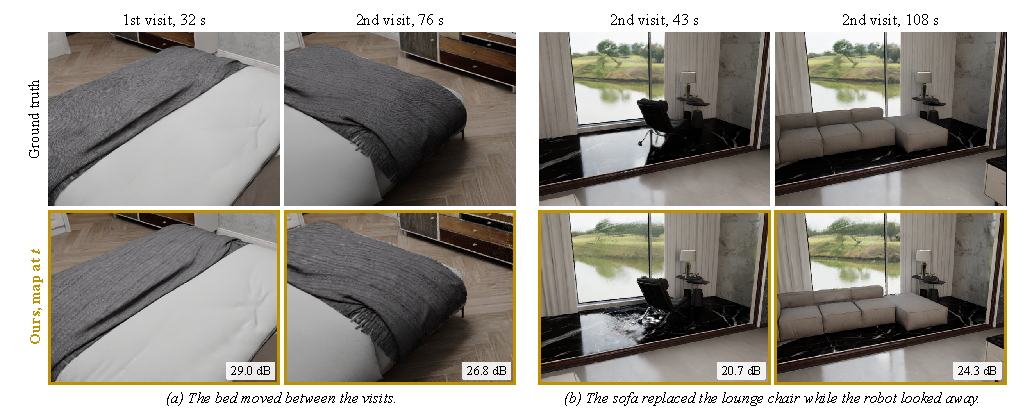
\includegraphics[width=\textwidth]{figures/fourd.pdf}
\caption{\textbf{Querying earlier states of the same scene.} Ground-truth frames and our Gaussian map queried at
the corresponding times. Left: the bed changes between visits. Right: the chair is replaced by the sofa within
the second visit. Historical queries retain the earlier object configuration while current queries show its replacement.}
\label{fig:supp_history}
\end{figure*}

\Cref{fig:supp_history} illustrates queries before and after changes within a visit and across visits.
The queried geometry is selected from the stored lifetimes; closed states remain available for their earlier times.
